\chapter{Sensitivity}
\label{sec:Appendix_sens} 
A discussion regarding the search sensitivity was carried out in the paper~\cite{HiggsBosonDecaysToQuarkonia}. The sensitivity of the measurement can be approximated by $\sqrt{S+B}/S$, where the S and B refer to as the number of signal and background events, respectively. The numerator indicates the statistical uncertainty of the observed events. As a reference, in the Run1 $H\to\gamma\gamma$ search, which contributed to the observation of the Higgs boson, the sensitivity was $\sim 0.11$~\cite{Khachatryan:2014ira}. In our search, the sensitivity of the Higgs boson decay is 242.1, where that of the Z boson decay is 15.1. A powerful background rejecting strategy while keeping high signal efficiency is worth developing in order to further improve the sensitivity. 

\begin{figure}[!ht]
  \begin{center}
    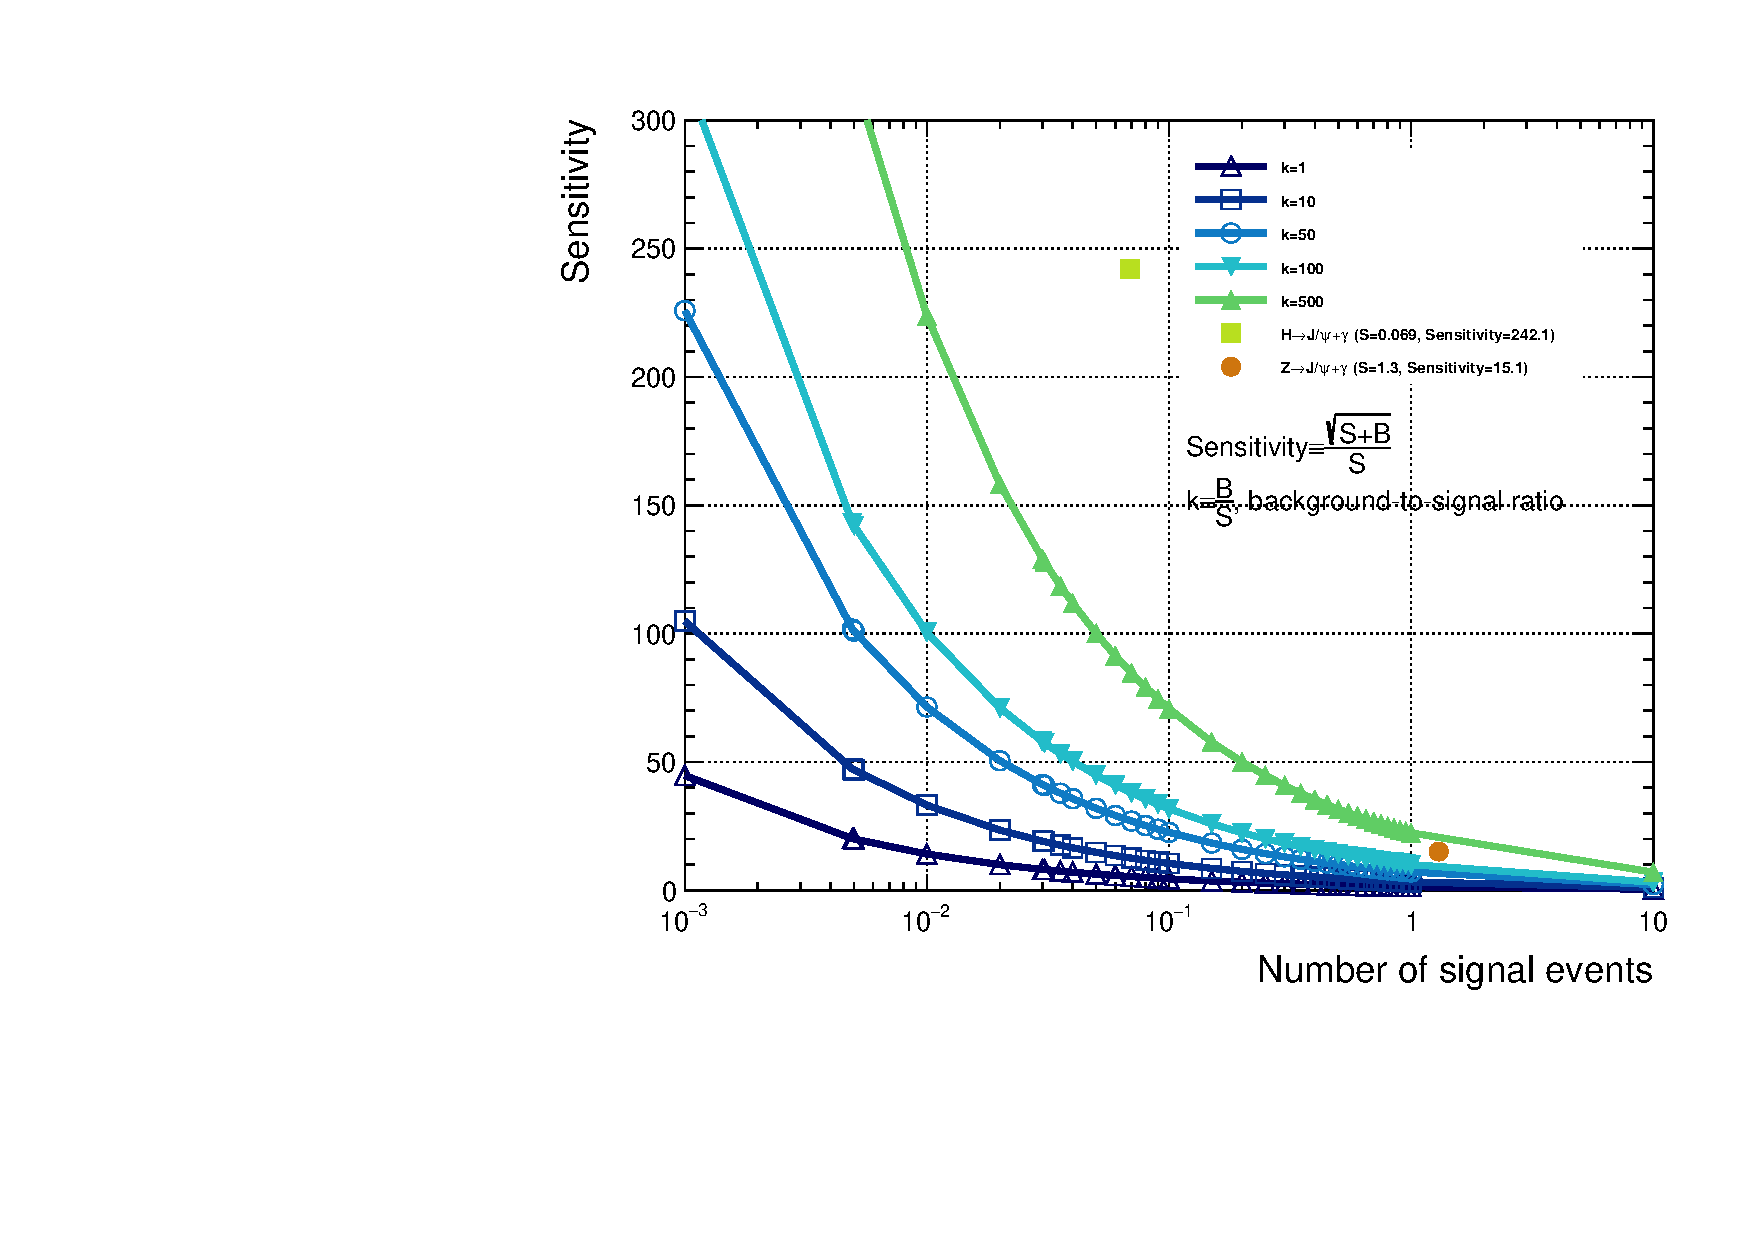
\includegraphics[width=0.95\textwidth]{Fig/Sensitivity_scan}\\
    \caption{The search sensitivity estimated from the Higgs(Z)$\to (J/\psi)\gamma$ decay.}
    \label{fig:Sensitivity}
  \end{center}
\end{figure}